\chapter{Rätselseite}

\raggedcolumns
\begin{multicols}{2}
	\section*{Mini-Sudoku}
	Trage in jede Zeile und Spalte die Ziffern 1, 2, 3,~4 so ein, dass A~waagrecht, A~senkrecht, B~senkrecht und F~senkrecht Primzahlen sind!

	\begin{center}
		\begin{tabular}{ |p{0.5cm}|p{0.5cm}|p{0.5cm}|p{0.5cm}| }
		\hline
		  a & b & c & d \\[0.5cm]
		\hline
		  e &   &   &   \\[0.5cm]
		\hline
		  f &   &   &   \\[0.5cm]
		\hline
		  g &   &   &   \\[0.5cm]
		\hline
		\end{tabular}
	\end{center}

	\section*{Altersrätsel}
	
	Zwei Mathematiker treffen sich zufällig auf der Straße und kommen ins Gespräch:\\
	- Hattest du nicht drei Söhne? Wie alt sind die denn jetzt?\\
	- Wenn man ihre Jahre zusammenzählt, erhält man 13 und wenn man sie miteinander multipliziert,
 	erhält man das heutige Datum.\\
	- Hmm, das genügt mir noch nicht \ldots}\\
	- Achja stimmt, ich hatte vergessen zu erwähnen, dass mein ältester Sohn einen Hund hat!\\
	- Danke, jetzt weiß ich ihr Alter.\\

	\emph{Wie alt sind die Söhne?}

		\columnbreak
		\columnbreak
	\section*{Kreuzzahlenrätsel}
	Jede Summe, und jeder Summand innerhalb der Summe, darf nur einmal auftreten.

	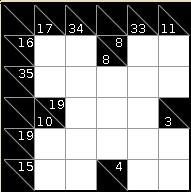
\includegraphics[width=0.9\linewidth]{2011-10-02-134837_191x192_scrot.png}

	\section*{Filmrätsel}
	Welchen Film haben wir hier versteckt?
	\begin{quote}
		\begin{tabular}{cccccccc}
			T & U & S & N & L & A & U & E \\
			Z & A & C & T & A & B & S & I \\
			N & O & H & K & R & A & V & S \\
			A & M & E & D & D & D & E & L \\
			T & W & O & E & E & L & O & W \\
			O & I & V & R & R & P & A & N \\
			R & A & M & S & S & S & K & C \\
		\end{tabular}
	\end{quote} 

	\end{multicols}
	\newpage
	\begin{multicols}{2}
	\section*{Minesweeper}
	Ein Spiel welches wohl keiner Erklärung mehr bedarf. Jedes Level ist eindeutig lösbar.

	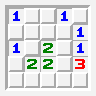
\includegraphics[width=0.45\linewidth]{minepuzzle_gen02tr.png}
	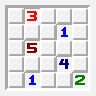
\includegraphics[width=0.45\linewidth]{minepuzzle_gen14tr.png}

	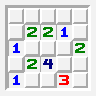
\includegraphics[width=0.45\linewidth]{minepuzzle_gen18tr.png}
	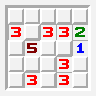
\includegraphics[width=0.45\linewidth]{minepuzzle_gen21tr.png}

	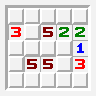
\includegraphics[width=0.45\linewidth]{minepuzzle_gen29tr.png}
	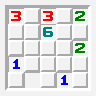
\includegraphics[width=0.45\linewidth]{minepuzzle_gen19tr.png}

	\section*{Visitenkarten}
	Welchen Anagramm-Beruf haben diese Personen?\\

	\begin{itemize}
		\item[]{Hanne Rubbich -- Ilztal}
		\item[]{Richie Hersvogt -- Zell}
		\item[]{Meike Schmettelin -- Berlin}
	\end{itemize}

	%\centerline{Hanne Rubbich \textendash{} Ilztal\\[0.2cm]}
	%\centerline{Richie Hersvogt \textendash{} Zell\\[0.2cm]}
	%\centerline{Meike Schmettelin \textendash{} Berlin\\[0.2cm]}

	\columnbreak
	\section*{Shikaku}

	Teile das Gitter in Rechtecke, sodass jedes Rechteck genau eine Nummer beinhaltet.
	Die Nummer gibt die Anzahl der Felder an, die das jeweilige Rechteck beinhaltet.

	\renewcommand{\arraystretch}{1.4}
	\begin{center}
		\arrayrulecolor{black!20} % Linienfarbe
		\begin{tabular}{|*{10}{p{0.2cm}|}}
		\hline
		 	 & 4 &   &  &  &   &  &   &   & 6\\\hline
 			4&   &   &  &  & 3 &  & 6 &  &  \\ \hline
 			 &   & 2 &  &  &   & 4&   &  & \\ \hline
 			 & 6 &   &  &  &   &  & 6 &  & \\ \hline
 			 &   &   & 8&  &   &  &   &  & \\ \hline
 			 &   & 4 &  &  &   &  &   &  & \\ \hline
 			 &   &   &  &  &   & 6&   &  & 2 \\ \hline
			 &   &   &  &  & 4 &  &   & 4& \\ \hline
 			 & 9 &   &  & 4&   &  &   &  & 6\\ \hline
			6&   &   &  &  & 6 &  &   & 4& \\ \hline
			 & 6 &   &  &8 &   &  &   &  & \\ \hline
 			9&   &   & 4&  &   &  &   &  & \\ \hline
 			 &   &   &  &  &   &  & 4 &  & \\ \hline
 			 &   &   &  &  &   & 9&   &  & \\ \hline
 			 &   & 4 &  &  &   &  &   & 4& \\ \hline
 			 &   &   & 4&  &   &  & 3 &  & \\ \hline
 			 &   & 6 &  & 3&   &  &   &  & 2\\ \hline
 			4&   &   &  &  &   &  &   & 6& \\ \hline
		\end{tabular}
		\arrayrulecolor{black}
	\end{center}
	\renewcommand{\arraystretch}{1}	
\end{multicols}
